\documentclass{IEEEtran}
\usepackage{cite}
\usepackage{authblk}
\usepackage{hyperref}
\usepackage{graphicx}
\usepackage{textgreek}

\graphicspath{{images/}}

\newcommand{\mailtodomain}[1]{\href{mailto:#1@nu.edu.kz}{\nolinkurl{#1}}}
\setlength{\parskip}{1em}

\begin{document}

\title{Malfunctioning engine clamping components detection using Phase-based video magnification}

\author[1]{Anuar Maratkhan}
\author[2]{Kudaibergen Urinbayev}
\author[1]{Ibrakhim Ilyassov}
\affil[1]{Department of Computer Science}
\affil[2]{Department of Robotics and Mechatronics}
\affil[1,2]{Nazarbayev University \protect\\
53 Qabanbay Batyr Ave., 010000 \protect\\
Astana, Kazakhstan \protect\\
Email: \texttt{\{\mailtodomain{anuar.maratkhan}, \mailtodomain{kudaibergen.urinbayev}, \mailtodomain{ibrakhim.ilyassov}\}@nu.edu.kz}}

\maketitle

\begin{abstract}
Human visual system has some limitations. While human can recognize some vivid oscillations such as leave swings on the wind, some of subtle fluctuations like pulse or sway of bridge left unperceivable for the naked eye. However, small changes in motion could contain essential information of the system and could be quantitively and qualitatively analyzed. These analysis are done through a video magnification that we are applying for engine mount inspection in our work.
\end{abstract}

\section{Introduction}

Human visual system has some limitations. While human can recognize some vivid oscillations such as leave swings on the wind, some of subtle fluctuations like pulse or sway of bridge left unperceivable for the naked eye. However, small changes in motion could contain essential information of the system and could be quantitively and qualitatively analyzed. These analysis are done through a video magnification that we are applying for engine mount inspection in our work.

Several video magnification techniques were proposed. In 2005, Lie et al suggested Lagrangian approach to amplify motions where pixels are tracked and motion vectors are amplified directly to synthesize videos with larger motions. This method required motion segmentation and manual correction of filling the holes after video processing \cite{Liu:2005:MM:1073204.1073223}.

\begin{figure}[h]
	\centering
	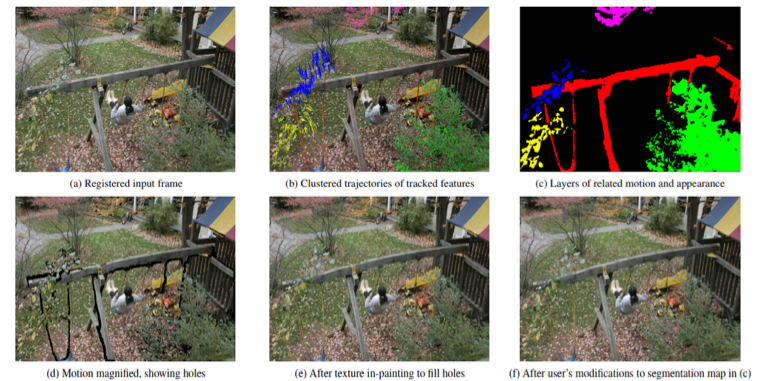
\includegraphics[width=0.5\textwidth]{Liu}
	\caption{Summary of motion magnification processing steps \cite{Liu:2005:MM:1073204.1073223}}
	\label{fig:Liu}
\end{figure}

Further, in 2012 a new magnification method was proposed that used Eulerian approach. Eulerian Video Magnification (EVM) computational method of a video amplification of subtle motions and color changes over time \cite{Wu:2012:EVM:2185520.2185561}. The main feature of this method is that instead of tracking and shifting each pixel explicitly as in Lagrangian approach Eulearian method operates with the color change of the pixel in the temporal domain. Therefore, due to EVM subtle color changes as well as the slight motions could be magnified.

The figure below describes the working principle of the EVM algorithm. Firstly, the video goes through the spatial decomposition to obtain spatial frequency bandwidth using Laplacian pyramids to decrease noise and allow to operate with small structures. The band-pass filter then applied to remove noise and inappropriate artefacts. Each pixel goes through temporal processing where the intensity is magnified by some factor. Afterwards video goes through reconstruction.

\begin{figure}[h]
	\centering
	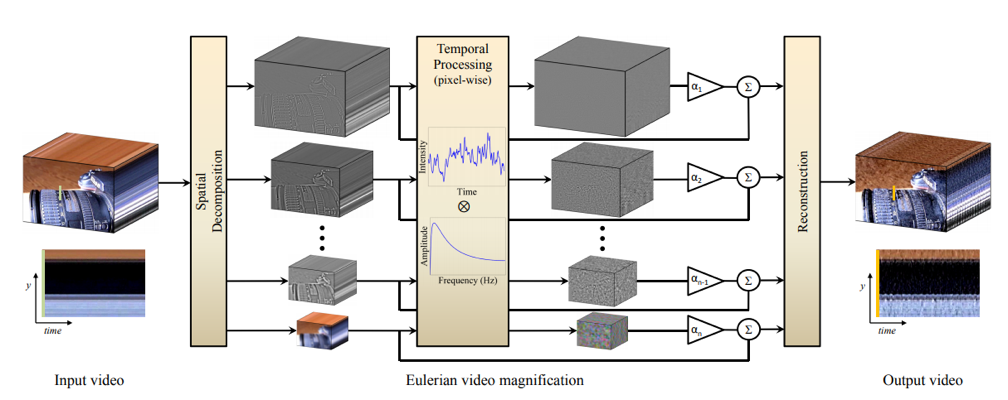
\includegraphics[width=0.5\textwidth]{EVM}
	\caption{Overview of the Eulerian video magnification framework. The system first decomposes the input video sequence into different spatial frequency bands, and applies the same temporal filter to all bands. The filtered spatial bands are then amplified by a given factor α, added back to the original signal, and collapsed to generate the output video. The choice of temporal filter and amplification factors can be tuned to support different applications. For example, we use the system to reveal unseen motions of a Digital SLR camera, caused by the flipping mirror during a photo burst (camera; full sequences are available in the supplemental video). Referenced from \cite{Wu:2012:EVM:2185520.2185561}}
	\label{fig:EVM}
\end{figure}

Thus, the change in the pixel intensity allows to amplify motion in spatial domain.

However, EVM method has its own drawback due to the linearity: noises are amplified gradually with motion magnification as well as some visual artefacts become visible in a fields of high frequency motions.

\section{Phase-based Video Magnification}

\begin{figure}[h]
	\centering
	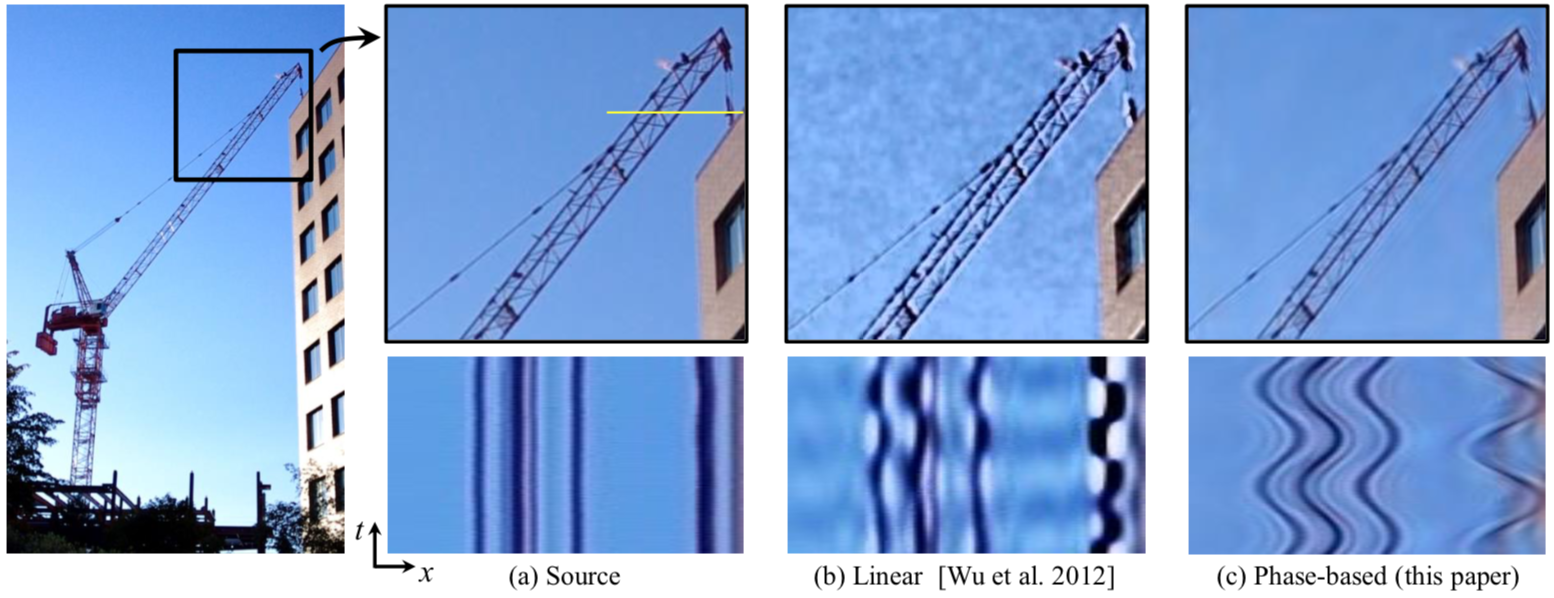
\includegraphics[width=0.5\textwidth]{phase-based}
	\caption{Motion magnification of a crane imperceptibly swaying in the wind. (a) Top: a zoom-in onto a patch in the original sequence (crane) shown on the left. Bottom: a spatiotemporal XT slice of the video along the profile marked on the zoomed-in patch. (b-c) Linear [Wu et al. 2012] and phase-based motion magnification results, respectively, shown for the corresponding patch and spatiotemporal slice as in (a). The previous, linear method visualizes the crane’s motion, but amplifies both signal and noise and introduces artifacts for higher spatial frequencies and larger motions, shown by the clipped intensities (bright pixels) in (b). In comparison, our new phase-based method supports larger magnification factors with significantly fewer artifacts and less noise (c). The full sequences are available in the supplemental video. Referenced from \cite{Wadhwa:2013:PVM:2461912.2461966}}
	\label{fig:phase-based}
\end{figure}

In the Fourier transform domain the amplitude of the sinusoids depends on amplitude of the basis function, while the change in phase corresponds to translation of the sinusoid. However, Fourier shift theorem works on the global motion, whereas in most cases only certain motions need to be magnified. Therefore, concept of localized Fourier series is introduced and it could be explained by Complex Steerable Pyramids.

\subsection{Complex Steerable Pyramids}
The steerable pyramid \cite{119725} is an overcomplete transform that decomposes an image according to spatial scale, orientation, and position. We understand this work as a way to do local Fourier transform for certain bandpassed frequencies.

The steerable pyramid \cite{119725} is an overcomplete transform that decomposes an image according to spatial scale, orientation, and position. We understand this work as a way to do local Fourier transform for certain bandpassed frequencies. The steerable pyramid method mentioned above is used to measure local amplitude and phase, which are exploit in \cite{Wadhwa:2013:PVM:2461912.2461966} to process motion. Those phases are then magnified by α. These works are replicated in our work for further use in engine mount test through video magnification that is unseen to the naked eye.

\begin{figure}[h]
	\centering
	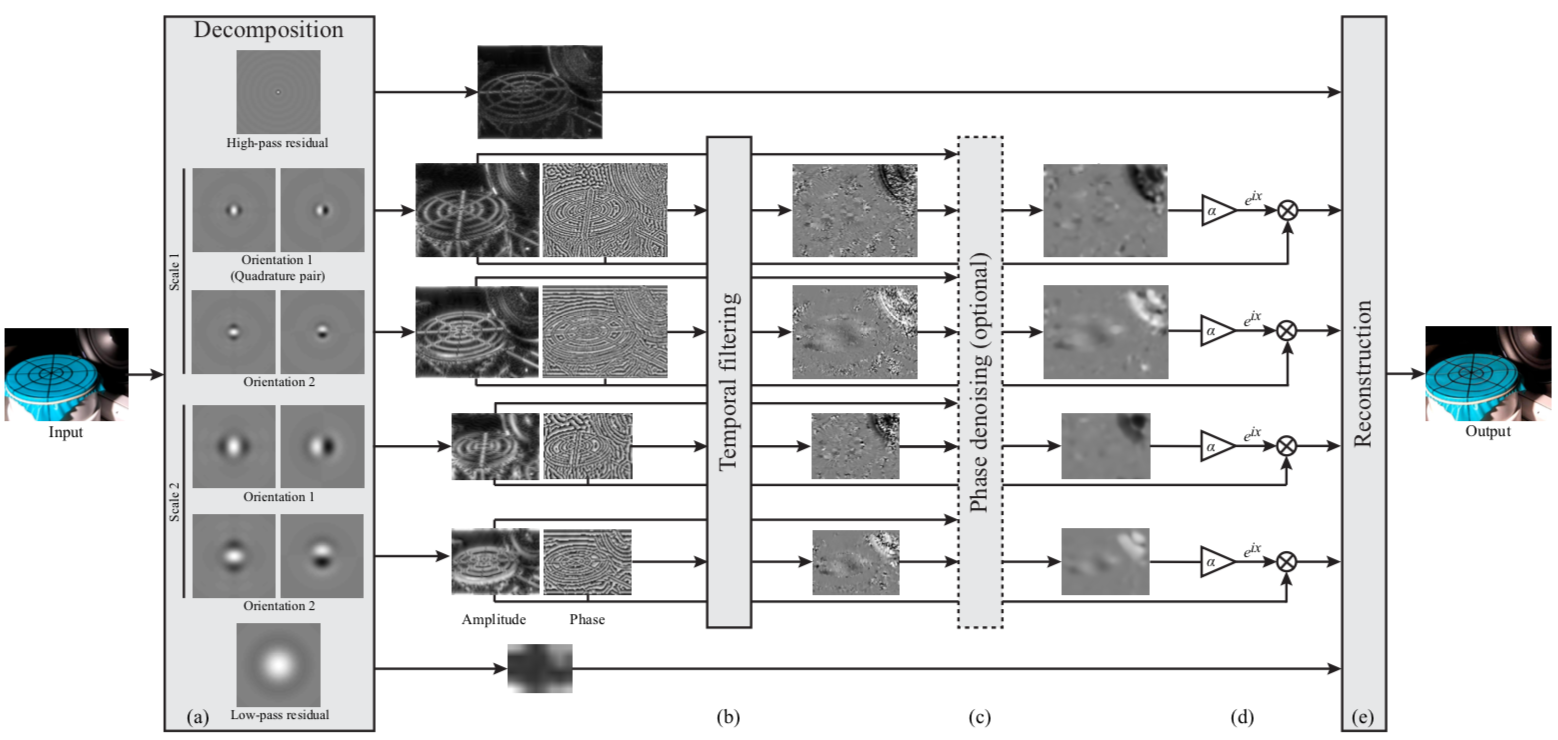
\includegraphics[width=0.5\textwidth]{phases}
	\caption{Our phase-based approach manipulates motion in videos by analyzing the signals of local phase over time in different spatial scales and orientations. We use complex steerable pyramids to decompose the video and separate the amplitude of the local wavelets from their phase (a). We then temporally filter the phases independently at at each location, orientation and scale (b). Optionally, we apply amplitude-weighted spatial smoothing (c, Sect. 3.4) to increase the phase SNR, which we empirically found to improve the results. We then amplify or attenuate the temporally-bandpassed phases (d), and reconstruct the video (e). This example shows the processing pipeline for the membrane sequence (Sect. 4), using a pyramid of two scales and two orientations (the relative difference in size between the pyramid levels is smaller in this figure for clarity of the visualization). Referenced from \cite{Wadhwa:2013:PVM:2461912.2461966}}
	\label{fig:phases}
\end{figure}

Figure above demonstrates the working principle of the Phase Based video magnification method. The main difference between just mentioned method and EVM is that the in video processing.

\section{Experimental setup}

To test given method the video of car engine was filmed. The video was shoot with the 25 fps Canon 550D. Due to the limited resources and time, video of car engine of Toyota Yaris (manufactured in 2011) was taken outdoor in cloudy/windy weather condition. 

Since car mount deinstallation and reinstallation required special tools and some mechanical engineering skills  it was decided to remove one of the spark plugs because according to \url{https://www.carsdirect.com/car-repair/5-causes-of-engine-vibration} worn out spark plugs is a common reason of the motor vibrations. 

\section{Usage}

We divide the work done into two parts (MATLAB and Python) because codes are separately written in MATLAB and Python programming languages. The MATLAB part is taken from original work of \cite{Wadhwa:2013:PVM:2461912.2461966}, and is used to magnify the video. On the other hand, the second part uses the output video from the first part and compares the video of properly working engine with the video of engine with defects in engine's mounts. The both parts are described in detail below.

\subsection{MATLAB code}

The original MATLAB code from \cite{Wadhwa:2013:PVM:2461912.2461966} has been used to magnify the video of working car engine. The proper usage of the part is described below.

\subsubsection{Input videos}

To add videos that are going to be magnified, you need to add video files inside \texttt{input\_files} directory inside main \texttt{MATLAB} directory. Further, the videos will be taken from this directory.

\subsubsection{Processing the video}

In order to magnify the chosen video, you need to run MATLAB function in the main MATLAB directory with the name \texttt{robt310\_final\_project}. The function accepts one argument - the name of the file (as a string). So, to run the video magnification method, call a function from terminal like this:

\texttt{robt310\_final\_project('video.mp4');}

In case you want to customize the function itself, change the function paramaters inside it. The parameters are set to process car engine, as in the example code of \cite{Wadhwa:2013:PVM:2461912.2461966} work. Default setting that can be customized are:

\begin{itemize}
	\item{\texttt{samplingRate} - the rate the video frames will be sampled. Higher the rate, slower the video play will be. We have decreased the original 400 down to 120 sampling rate because the original work has been processing the video with 400 fps compared to our 25 fps.}
	\item{\texttt{loCutoff} and \texttt{hiCutoff} - the range of low and high frequencies (Hz) to be bandpassed for magnification. The default parameters \texttt{loCutoff} = 15, and \texttt{hiCutoff} = 25 has not been changed from the original code.}
	\item{\texttt{alpha} - $\alpha$ rate according to which the video will be magnified. Higher the alpha, more the video will be magnified. The original work magnified the video with $\alpha$ = 15. We are magnifying it with $\alpha$ = 50 in order to see the magnification more clearly.}
	\item{\texttt{sigma} - parameter that is used in the magnification. Changing the alpha will result in the magnification style. We set it to default 3 as in the original code.}
	\item{\texttt{pyrType} - default set is 'octave'. Another option to use is 'halfOctave' which is said to produce different result and uses more computational resources. The parameter comes from complex steerable pyramids and is out of scope of our work. Thus, we have used the default value 'octave'.}
\end{itemize}

The only recommended change is the \texttt{samplingRate} parameter that changes the video look in time according to number of frames per second (fps) in the video to be processed.

\subsubsection{Output videos}

The output files will be saved in \texttt{output\_files} directory. The names of the files are set in code by using the original input filename, and the parameters used to process the video.

\subsection{Python code}

\subsubsection{Matching frames of videos}

There exist a problem that two videos, original and defected one, can move with shifted frames. For example, first video’s engine can go up and second video’s engine can go down, so they are moving in different phases. Therefore, it will be wrong without initial matching of videos to calculate RMSE.

First of all, we cut a rectangular region with engine from video using special GUI. Cropped image is used as template in order to find the region with this template in both videos. Thus, we found the maximum upper deviation in both videos by using locations of detected regions based on provided template. The first frame, where is maximum upper deviation occurs, will be used in order to match with the first frame of the second video, which has maximum upper shift of engine. We have written a function \texttt{getFirst()} in \texttt{match.py}  module that returns pair value of first frame and upper boundary of engine shift. 

\subsubsection{Calculating RMSE}

After matching of two videos by frames, we calculated RMSE for every frame and get the mean of all values for every frame. Thus, the resulting RMSE is \textbf{7.49}.

\subsubsection{Usage for calculating RMSE}

\paragraph{Cropping a template image}

Firstly, we need to crop a region with engine in order to match videos by frames. 
You need to call a python script and pass video’s name as argument:

Example:

\texttt{\$ python crop.py engine.mp4 }

Secondly, select region by clicking and cropping using GUI:

\begin{figure}[h]
	\centering
	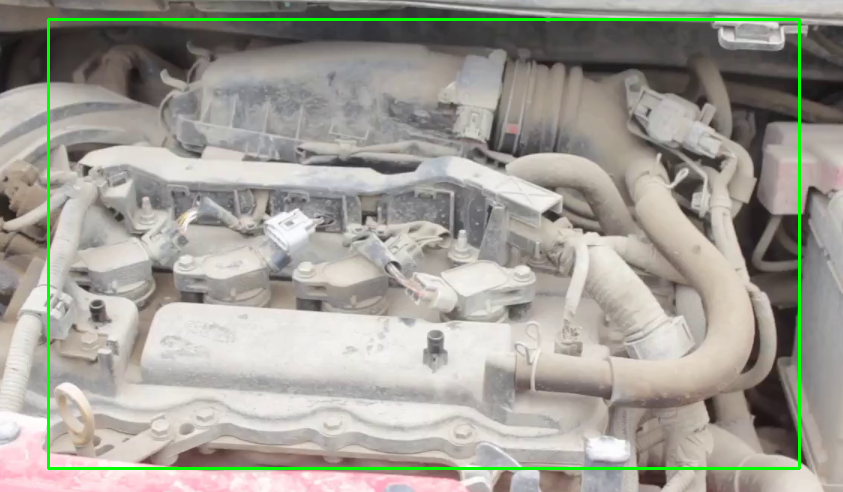
\includegraphics[width=0.5\textwidth]{RMSE}
	\label{fig:RMSE}
\end{figure}

Then, press ‘c’ key in order to cut and save as template in ‘roi.jpg’ file.

\paragraph{Calculating RMSE}

Run python script and pass two videos’ filenames as arguments in order to compare them. 
Example:

\texttt{\$ python calculate.py 1.avi 2.avi}

\section{Results}

We used phase based motion magnification and calculated RMSE for two videos: original and defected. Initially, RMSE of two videos was 7.62 without frame matching. The result with frame matching is 7.49. We could not identify the threshold in order to classify defected or not defected engines, because we have only one observation

\section{Conclusion}

In conclusion, even though the video was taken with 25 fps the resulting processed video sequence shown considerable difference between two videos: with and without one spark plug. The output RMSE shown 7.49. In order to achieve more accurate results in video magnification it is highly suggested to use high FPS video camera because the video amplifies more steadily. In addition, to achieve less errors in video comparing indoor shooting is highly advised because even subtle camera shaking highly reflected in the processed file.

\bibliographystyle{IEEEtran}
\bibliography{reference}
\printbibliography

\end{document}